% Untangling Federal Jurisdiction
% Part 3

% All content comes from Stephen Pratt. I have no idea if he approves of this effort or not.

\documentclass{beamer}
\usetheme{Madrid}
%\usetheme{Goettingen}
\usefonttheme{serif}
\usefonttheme{structuresmallcapsserif}
% \usepackage[font=small,labelfont=bf]{caption}
\usepackage{xcolor}
\usepackage{rotating}

\setbeamerfont{section title}{parent=title}
\setbeamercolor{section title}{parent=titlelike}
\defbeamertemplate*{section page}{default}[1][]
{
    \centering
    \begin{beamercolorbox}[sep=8pt,center,#1]{section title}
        \usebeamerfont{section title}\insertsection\par
    \end{beamercolorbox}
}
\newcommand*{\sectionpage}{\usebeamertemplate*{section page}}

\def\Put(#1,#2)#3{\leavevmode\makebox(0,0){\put(#1,#2){#3}}}

\makeatletter
\setbeamertemplate{footline}
{
    % Commented out to remove footer line entirely
%    \leavevmode%
%    \hbox{%
%    \begin{beamercolorbox}[wd=.333333\paperwidth,ht=2.25ex,dp=1ex,center]{author in head/foot}%
%        \usebeamerfont{author in head/foot}\insertshortauthor%~~\beamer@ifempty{\insertshortinstitute}{}{(\insertshortinstitute)}
%    \end{beamercolorbox}%
%    \begin{beamercolorbox}[wd=.333333\paperwidth,ht=2.25ex,dp=1ex,center]{title in head/foot}%
%        \usebeamerfont{title in head/foot}\insertshorttitle
%    \end{beamercolorbox}%
%    \begin{beamercolorbox}[wd=.333333\paperwidth,ht=2.25ex,dp=1ex,right]{date in head/foot}%
%        \usebeamerfont{date in head/foot}\insertshortdate{}\hspace*{2em}
%        \insertframenumber{} / \inserttotalframenumber\hspace*{2ex} 
%    \end{beamercolorbox}}%
%    \vskip0pt%
}
\makeatother

\newenvironment<>{varblock}[2][\textwidth]{
    \begin{center}
        \begin{minipage}{#1}
            \setlength{\textwidth}{#1}
            \begin{actionenv}#3
                \def\insertblocktitle{#2}
                \par
                \usebeamertemplate{block begin}}
            {\par
                \usebeamertemplate{block end}
            \end{actionenv}
        \end{minipage}
    \end{center}
}

\DeclareGraphicsExtensions{.pdf,.png,.jpg}


\begin{document}
\unitlength=1pt

\section{Life after Kleppe}
\frame{\sectionpage}

\begin{frame}{Gouvernor Morris and the Property Clause}
    \centering
    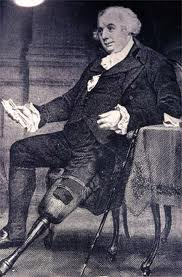
\includegraphics[height=.8\textheight]{img/morris-full.png} \\
\end{frame}

\begin{frame}
    \begin{columns}[onlytextwidth]
        \column{0.5\textwidth}
            \textbf{Letter, December 4, 1803} \\
            Morris, by his own admission, had attempted to concoct a deception,
            if not a fraud, hidden in duplicitous wording of the Property
            Clause.

        \column{0.5\textwidth}
            \centering
            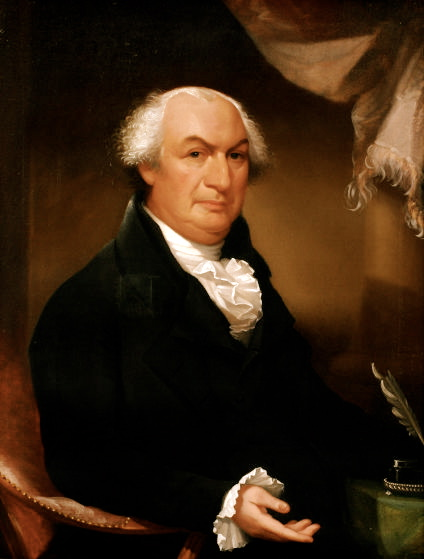
\includegraphics[width=0.95\textwidth]{img/morris-portrait.png} \\
            Gouvernor Morris, 1803 \\
    \end{columns}
\end{frame}

\begin{frame}
    \begin{columns}[onlytextwidth]
        \column{0.5\textwidth}
            \textbf{Letter, December 4, 1803} \\
            ``I went as far as circumstances would permit\ldots Had it been
            more pointedly expressed, a strong opposition would have been made.''

        \column{0.5\textwidth}
            \centering
            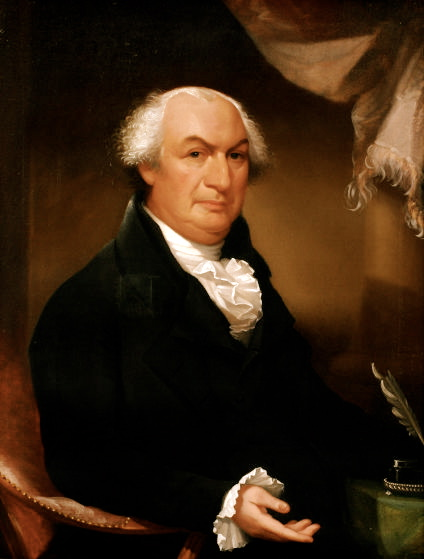
\includegraphics[width=0.95\textwidth]{img/morris-portrait.png} \\
            Gouvernor Morris, 1803 \\
    \end{columns}
\end{frame}

\begin{frame}{1976, Property Clause Revisited}
    \centering
    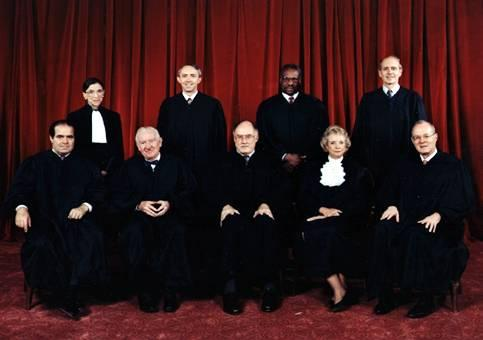
\includegraphics[width=0.75\textwidth]{img/sc-1976.png} \\
\end{frame}

\begin{frame}
    \begin{columns}[onlytextwidth]
        \column{0.5\textwidth}
            \centering
            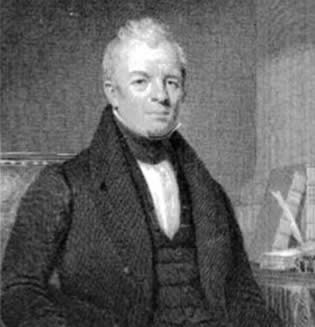
\includegraphics[width=0.95\textwidth]{img/james-kent.png} \\
            James Kent, 1826 \\
            \emph{Commentaries on American Law}, 4 vols. \\

        \column{0.5\textwidth}
            { \large ``[Judges] roam at large in the trackless field of their own imaginations.''}
    \end{columns}
\end{frame}

\begin{frame}{1976, Property Clause Revisited}
    \centering
    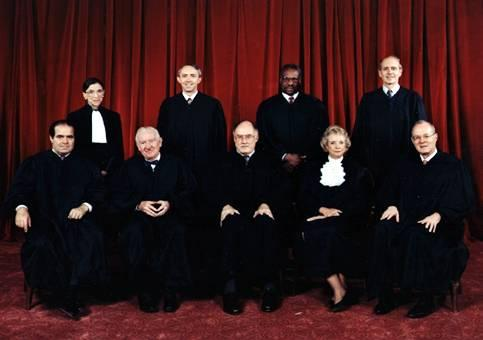
\includegraphics[width=0.75\textwidth]{img/sc-1976.png} \\
    ``\ldots make all needful rules and regulations\ldots'' \\
    \Put(260,60){
\includegraphics[width=.2\textwidth]{img/sherlock.png}}
\end{frame}

\begin{frame}{``Emanations from Penumbrae''}
   \centering
   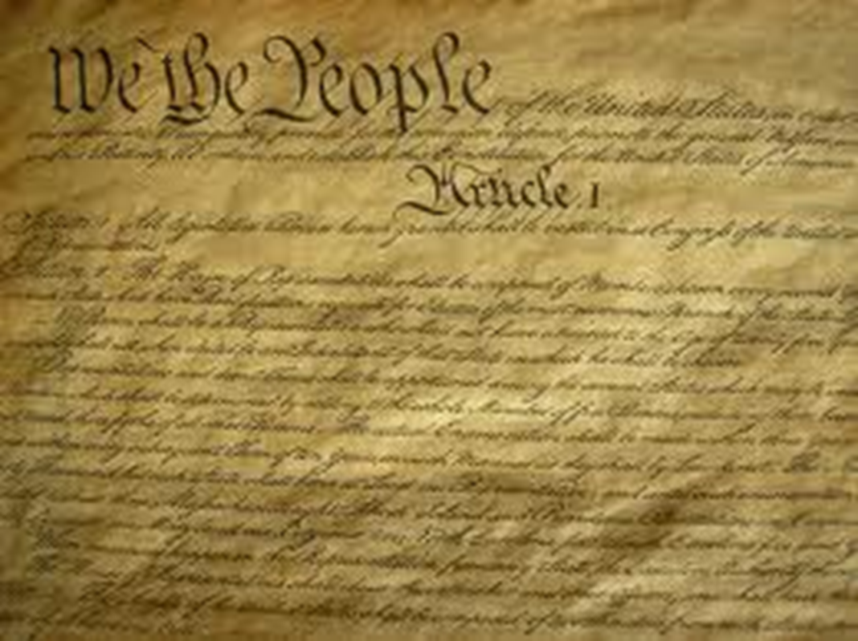
\includegraphics[height=.7\textheight]{img/constitution.png} \\
   \Put(200,080){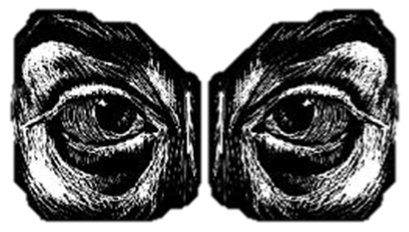
\includegraphics[width=.4\textwidth]{img/eyes.png}}
\end{frame}

\begin{frame}{``Emanations from Penumbrae''}
   \centering
   
\includegraphics[height=.7\textheight]{img/fire.png} \\
   \Put(200,080){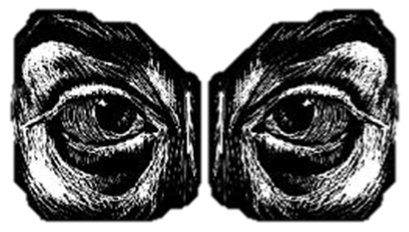
\includegraphics[width=.4\textwidth]{img/eyes.png}}
\end{frame}

\begin{frame}{Kleppe v. New Mexico, 1976}
    \centering
    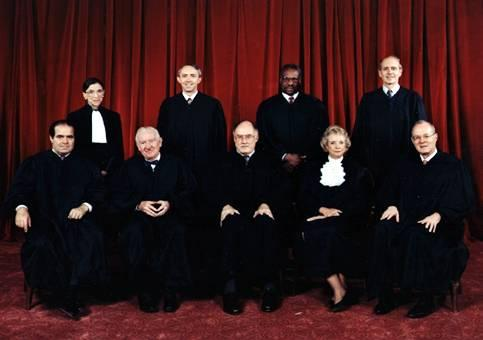
\includegraphics[width=0.75\textwidth]{img/sc-1976.png} \\
    { \large Federal legislative power over public lands is ``complete'' and
    ``without limitation.'' \\ }
    \Put(260,160){
\includegraphics[width=.2\textwidth]{img/sherlock.png}}
\end{frame}

\begin{frame}
    \begin{columns}[onlytextwidth]
        \column{0.5\textwidth}
            { \large Imagine Gouvernor Morris now\ldots }
        \column{0.5\textwidth}
            \centering
            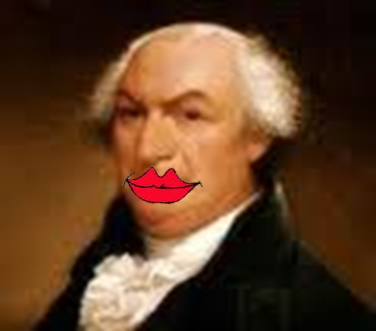
\includegraphics[width=0.95\textwidth]{img/morris-smile.png} \\
    \end{columns}
\end{frame}

\begin{frame}{Jurisdiction Clause Family --- Supremacy}
    \centering
    
\includegraphics[height=0.85\textheight]{img/family.png} \\
    \huge{\textbf{ \color{white}
        %\Put(25, 300){\begin{sideways}\colorbox{blue}{Admissions}\end{sideways}}
        %\Put(60, 300){\begin{sideways}\colorbox{blue}{Claims}\end{sideways}}
        %\Put(90, 300){\begin{sideways}\colorbox{blue}{Property}\end{sideways}}
        %\Put(134, 300){\begin{sideways}\colorbox{blue}{Guarantee}\end{sideways}}
        %\Put(168, 300){\begin{sideways}\colorbox{blue}{Enclave}\end{sideways}}
        %\Put(200, 300){\begin{sideways}\colorbox{blue}{Engagements}\end{sideways}}
        \Put(235, 300){\begin{sideways}\colorbox{blue}{Supremacy}\end{sideways}}
    }}
\end{frame}

\begin{frame}{Supremacy Clause}
   \centering
   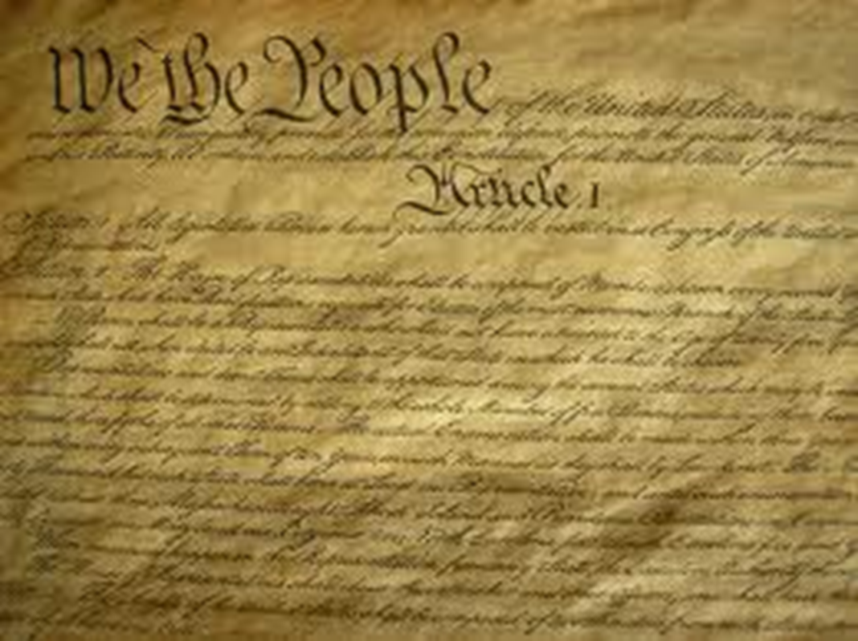
\includegraphics[height=.7\textheight]{img/constitution.png} \\
   \textbf{Article VI, clause 2:} ``This Constitution, and the Laws of the
   United States \emph{which shall be made in Pursuance thereof}\ldots shall be
   the supreme Law of the Land.''
\end{frame}

\begin{frame}{United States Senate and House of Representatives}
    \centering
    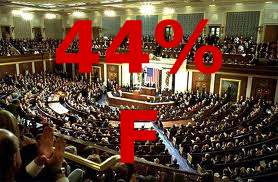
\includegraphics[width=0.75\textwidth]{img/house-senate-fail.png} \\
\end{frame}

\begin{frame}{Kleppe v. New Mexico, 1976}
    \centering
    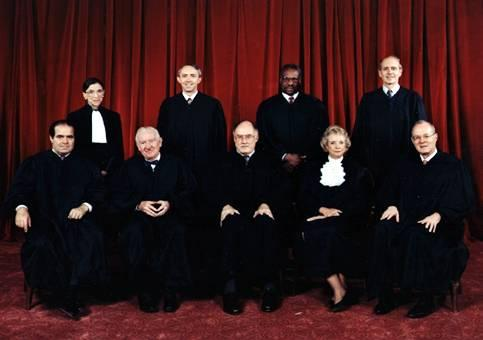
\includegraphics[width=0.65\textwidth]{img/sc-1976.png} \\
    Congress may enact legislation governing federal lands pursuant to the
    property clause and ``when Congress so acts, federal legislation
    necessarily overrides conflicting state laws under the \emph{supremacy
    clause}.''
\end{frame}

\begin{frame}{Continuum of \textbf{\emph{Sliding}} Judicial Opinions}
    \Put(20,20){\Large \begin{turn}{50} Johnson v. McIntosh, 1823 \end{turn}}
    \Put(50,10){\Large \begin{turn}{50} Benner v. Porter, 1850 \end{turn}}
    \Put(80,30){\Large \begin{turn}{50} Kohl v. United States, 1875 \end{turn}}
    \Put(110,45){\Large \begin{turn}{50} Ft. Leavenworth v. Lowe, 1885 \end{turn}}
    \Put(130,40){\Large \begin{turn}{50} Collins v. Yosemite Park, 1938 \end{turn}}
    \Put(170,30){\Large \begin{turn}{50} Kleppe v. New Mexico, 1976 \end{turn}}
    \Put(190,-115){\Large \begin{turn}{50} FPLMA, 1976 \end{turn}}
    {
        \color{red}
        \thicklines
        \Put(-20, -130){ \line(1, 0){250} }
    }
    \pause
    \Put(-30,100){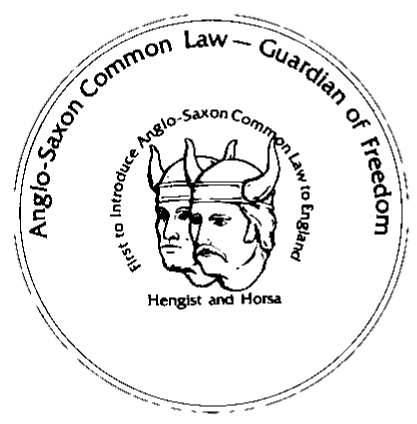
\includegraphics[width=.3\textwidth]{img/hh-coin.png}}
    \pause
    \Put(260,0){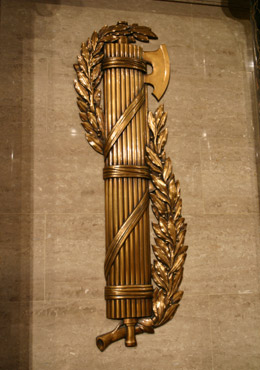
\includegraphics[height=.4\textheight]{img/fasces.png}}
    \pause
    \Put(30,-240){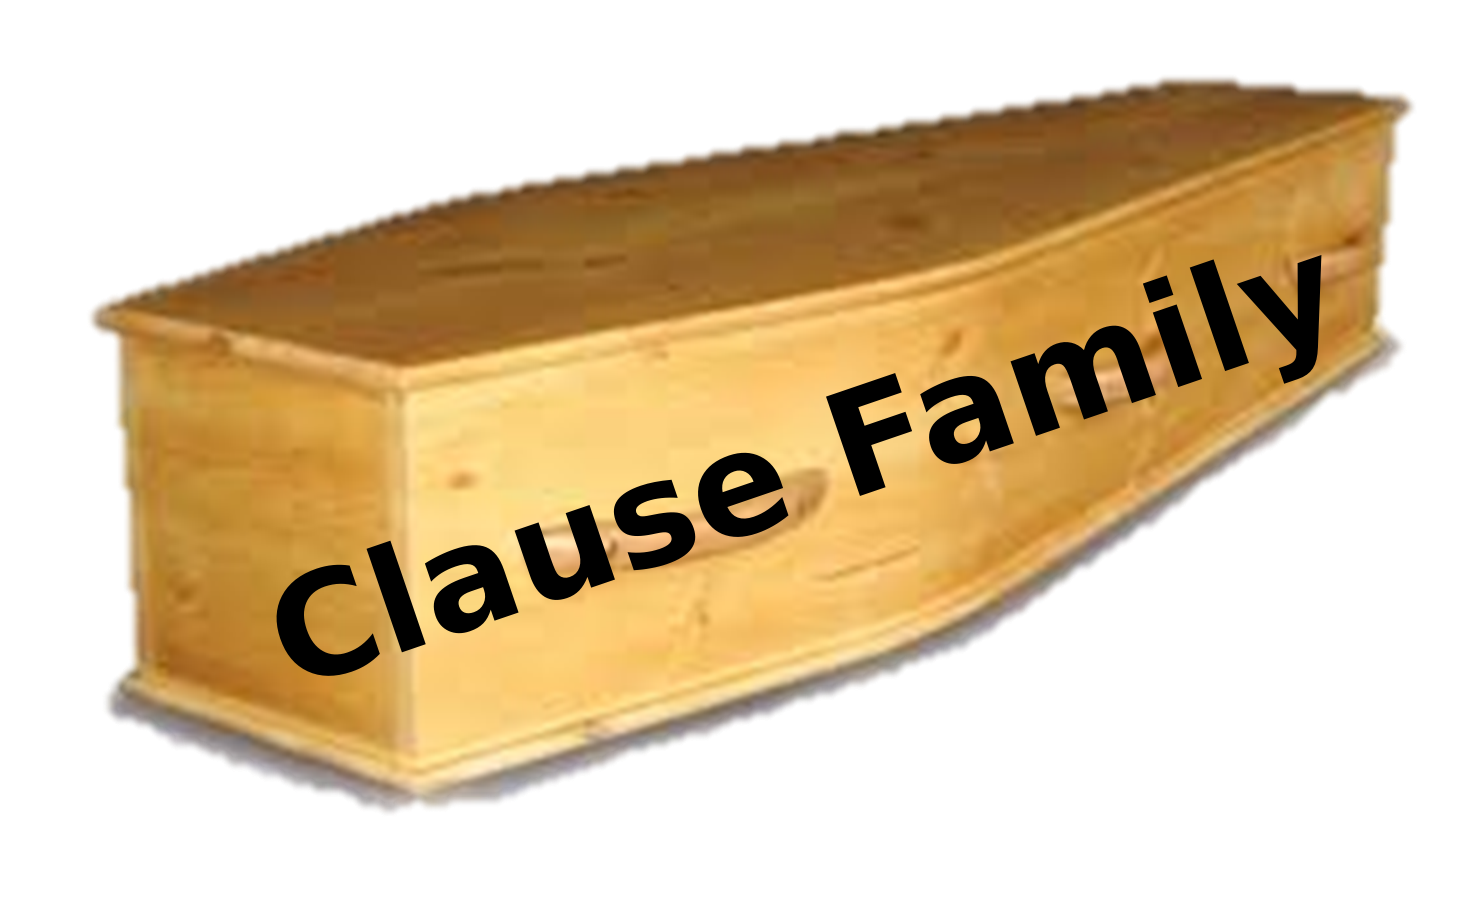
\includegraphics[width=.5\textwidth]{img/coffin-clause.png}}
\end{frame}

\begin{frame}{Here lies the Clause Family}
    \centering
    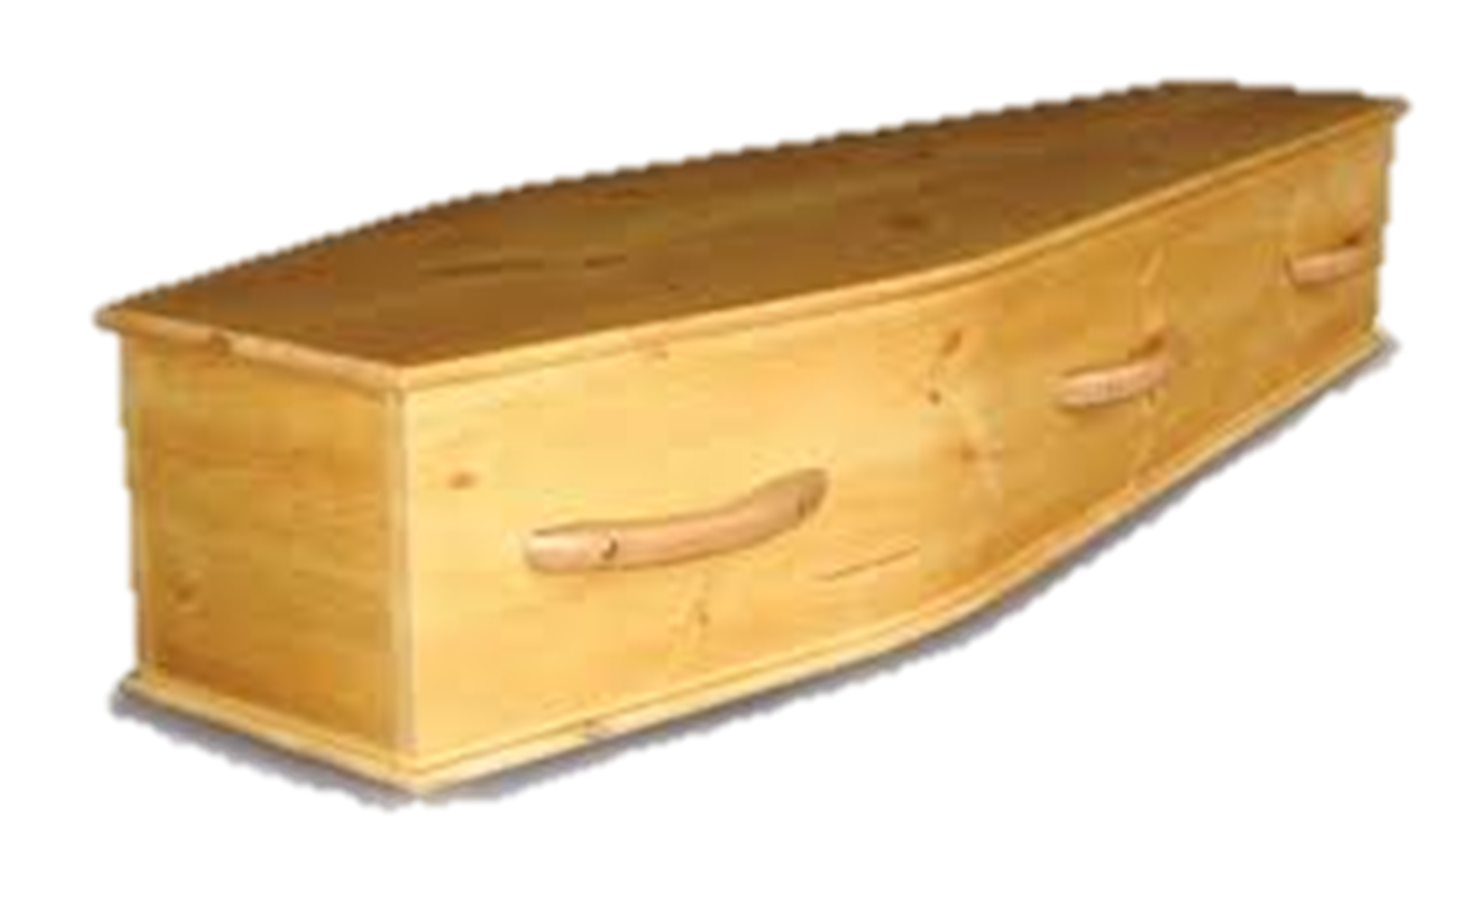
\includegraphics[width=.6\textwidth]{img/coffin.png} \\
    { \large
    Born March 4, 1789 \\
    Died by Strangulation, 1976 \\
    }
\end{frame}

\begin{frame}{126 Days after Kleppe: FLPMA}
    \centering
    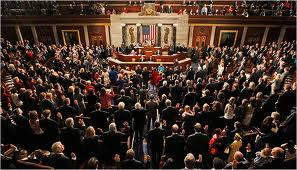
\includegraphics[width=.8\textwidth]{img/congress.png} \\
    Federal Lands Policy and Management Act \\
    { \large ``\ldots that it is the policy of the United States that the
    public lands be retained in Federal ownership\ldots'' }
\end{frame}

\begin{frame}
    
\includegraphics[width=.3\textwidth]{img/stop.png}
    \hspace{10pt}
    
\includegraphics[width=.3\textwidth]{img/think.png}
    \hspace{10pt}
    
\includegraphics[width=.3\textwidth]{img/wrong-way.png} \\
    \vspace{20pt}
    \begin{block}{Consequences of Kleppe}
        Public lands within the States have been rendered jurisdictionally equivalent to pre-statehood Territories, the District of Columbia, and federal enclaves!
    \end{block}
\end{frame}

\begin{frame}{Jurisdiction Clause Family --- Claims}
    \centering
    
\includegraphics[height=0.85\textheight]{img/family.png} \\
    \huge{\textbf{ \color{white}
        %\Put(25, 300){\begin{sideways}\colorbox{blue}{Admissions}\end{sideways}}
        \Put(70, 300){\begin{sideways}\colorbox{blue}{Claims}\end{sideways}}
        %\Put(90, 300){\begin{sideways}\colorbox{blue}{Property}\end{sideways}}
        %\Put(134, 300){\begin{sideways}\colorbox{blue}{Guarantee}\end{sideways}}
        %\Put(168, 300){\begin{sideways}\colorbox{blue}{Enclave}\end{sideways}}
        %\Put(200, 300){\begin{sideways}\colorbox{blue}{Engagements}\end{sideways}}
        %\Put(235, 300){\begin{sideways}\colorbox{blue}{Supremacy}\end{sideways}}
    }}
\end{frame}

\begin{frame}{Claims Clause}
   \centering
   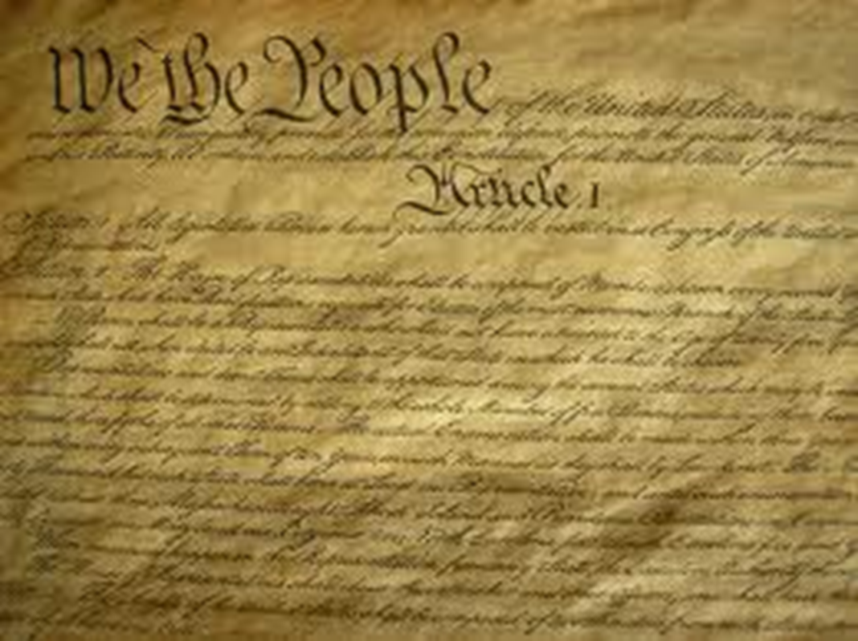
\includegraphics[height=.7\textheight]{img/constitution.png} \\
   \only<1>{\textbf{Article IV, sec. 3, cl. 2:} ``\ldots nothing in this Constitution shall be so construed as to Prejudice any \emph{claims}\ldots of any particular State.''}
   \only<2>{\textbf{Article IV, sec. 3, cl. 2:} \st{``\ldots nothing in this Constitution shall be so construed as to Prejudice any \emph{claims}\ldots of any particular State.''}}
\end{frame}

\begin{frame}{Engagements Clause}
   \centering
   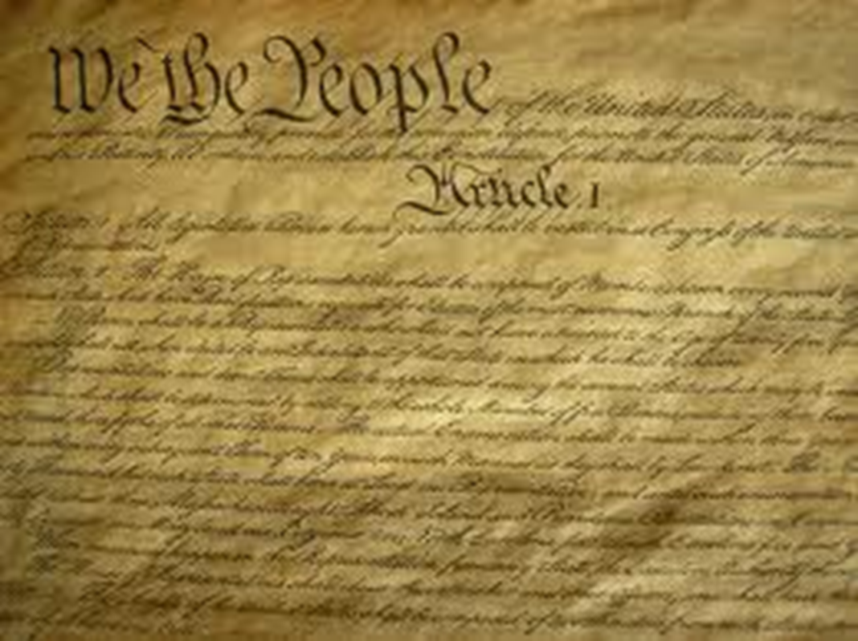
\includegraphics[height=.7\textheight]{img/constitution.png} \\
   \only<1>{\textbf{Article VI, clause 1:} ``All\ldots \emph{Engagements} entered into,
   before the Adoption of this Constitution, shall be as valid against the
   United States under this Constitution, as under the Confederation.''}
   \only<2>{\textbf{Article VI, clause 1:} \st{``All\ldots \emph{Engagements} entered into,
   before the Adoption of this Constitution, shall be as valid against the
   United States under this Constitution, as under the Confederation.''}}
\end{frame}

\begin{frame}{Engagements Clause}
   \centering
   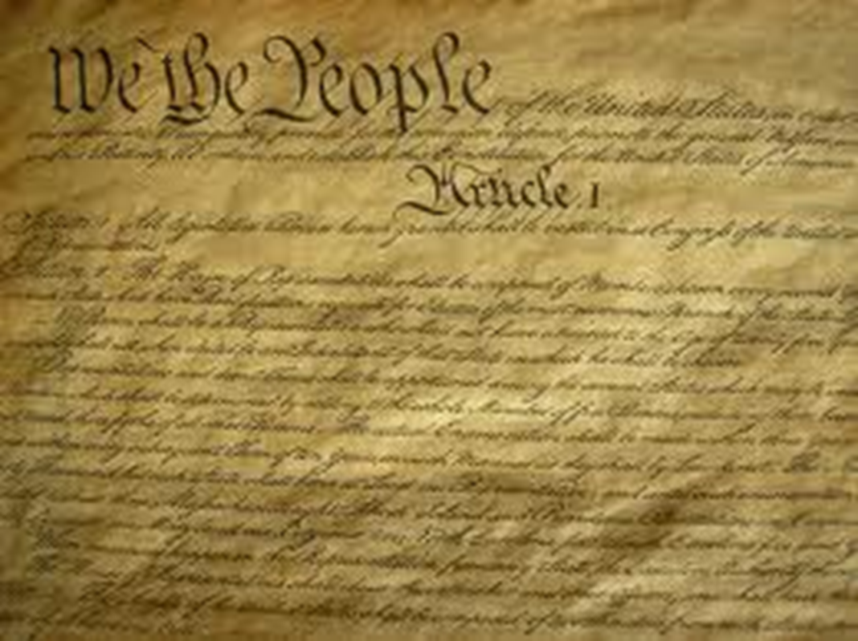
\includegraphics[height=.7\textheight]{img/constitution.png} \\
   By an act of Congress, the Constitution was amended by a change in policy to
   abandon the requirement to dispose of territorial and public land.
\end{frame}

\begin{frame}{Jurisdiction Clause Family}
    \centering
    
\includegraphics[height=0.85\textheight]{img/family.png} \\
    \huge{\textbf{ \color{white}
        \Put(25, 300){\begin{sideways}\colorbox{blue}{Admissions}\end{sideways}}
        \Put(60, 300){\begin{sideways}\colorbox{blue}{Claims}\end{sideways}}
        \Put(90, 300){\begin{sideways}\colorbox{blue}{Property}\end{sideways}}
        \Put(134, 300){\begin{sideways}\colorbox{blue}{Guarantee}\end{sideways}}
        \Put(168, 300){\begin{sideways}\colorbox{blue}{Enclave}\end{sideways}}
        \Put(200, 300){\begin{sideways}\colorbox{blue}{Engagements}\end{sideways}}
        \Put(235, 300){\begin{sideways}\colorbox{blue}{Supremacy}\end{sideways}}
    }}
\end{frame}

\begin{frame}{Jurisdiction Clause Family}
    \centering
    
\includegraphics[height=0.85\textheight]{img/family.png} \\
    \huge{\textbf{ \color{white}
        \Put(17, 300){ \begin{sideways}\colorbox{red}{\st{Admissions}}\end{sideways}}
        \Put(52, 300){ \begin{sideways}\colorbox{red}{\st{Claims}}\end{sideways}}
        \Put(82, 300){ \begin{sideways}\colorbox{red}{\st{Property}}\end{sideways}}
        \Put(134, 300){\begin{sideways}\colorbox{red}{\st{Guarantee}}\end{sideways}}
        \Put(168, 300){\begin{sideways}\colorbox{red}{\st{Enclave}}\end{sideways}}
        \Put(200, 300){\begin{sideways}\colorbox{red}{\st{Engagements}}\end{sideways}}
        \Put(235, 300){\begin{sideways}\colorbox{red}{\st{Supremacy}}\end{sideways}}
    }}
\end{frame}

\begin{frame}
    \centering
    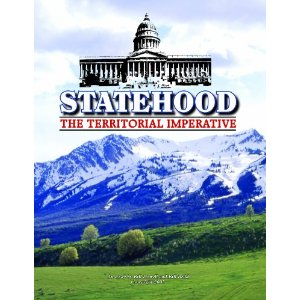
\includegraphics[height=.9\textheight]{img/territorial-imperative} \\
    Bill Howell, Bill Redd --- 2005, 524 pages \\
\end{frame}

\end{document}
